\newpage
\begin{table}
    \centering
    \caption{Atomic coordinates of Helical H$_2$ tetramer
 (\AA ngstroms)}
    \label{h2_4}
    \begin{tabular}{ c c c c }
    \hline
    \hline
    Atomic & & & \\
    Symbol & X & Y & Z \\
    \hline
	H &   0.000000 &   0.000000 &   0.000000 \\
	H &   0.750000 &   0.000000 &   0.000000 \\
	H &   0.000000 &   1.500000 &   0.000000 \\
	H &   0.375000 &   1.500000 &  -0.649520 \\
	H &   0.000000 &   3.000000 &   0.000000 \\
	H &  -0.375000 &   3.000000 &  -0.649520 \\
	H &   0.000000 &   4.500000 &  -0.000000 \\
	H &  -0.750000 &   4.500000 &  -0.000000 \\
    \hline
    \hline
    \end{tabular}
\end{table}
\newpage
\begin{figure}
\centering
    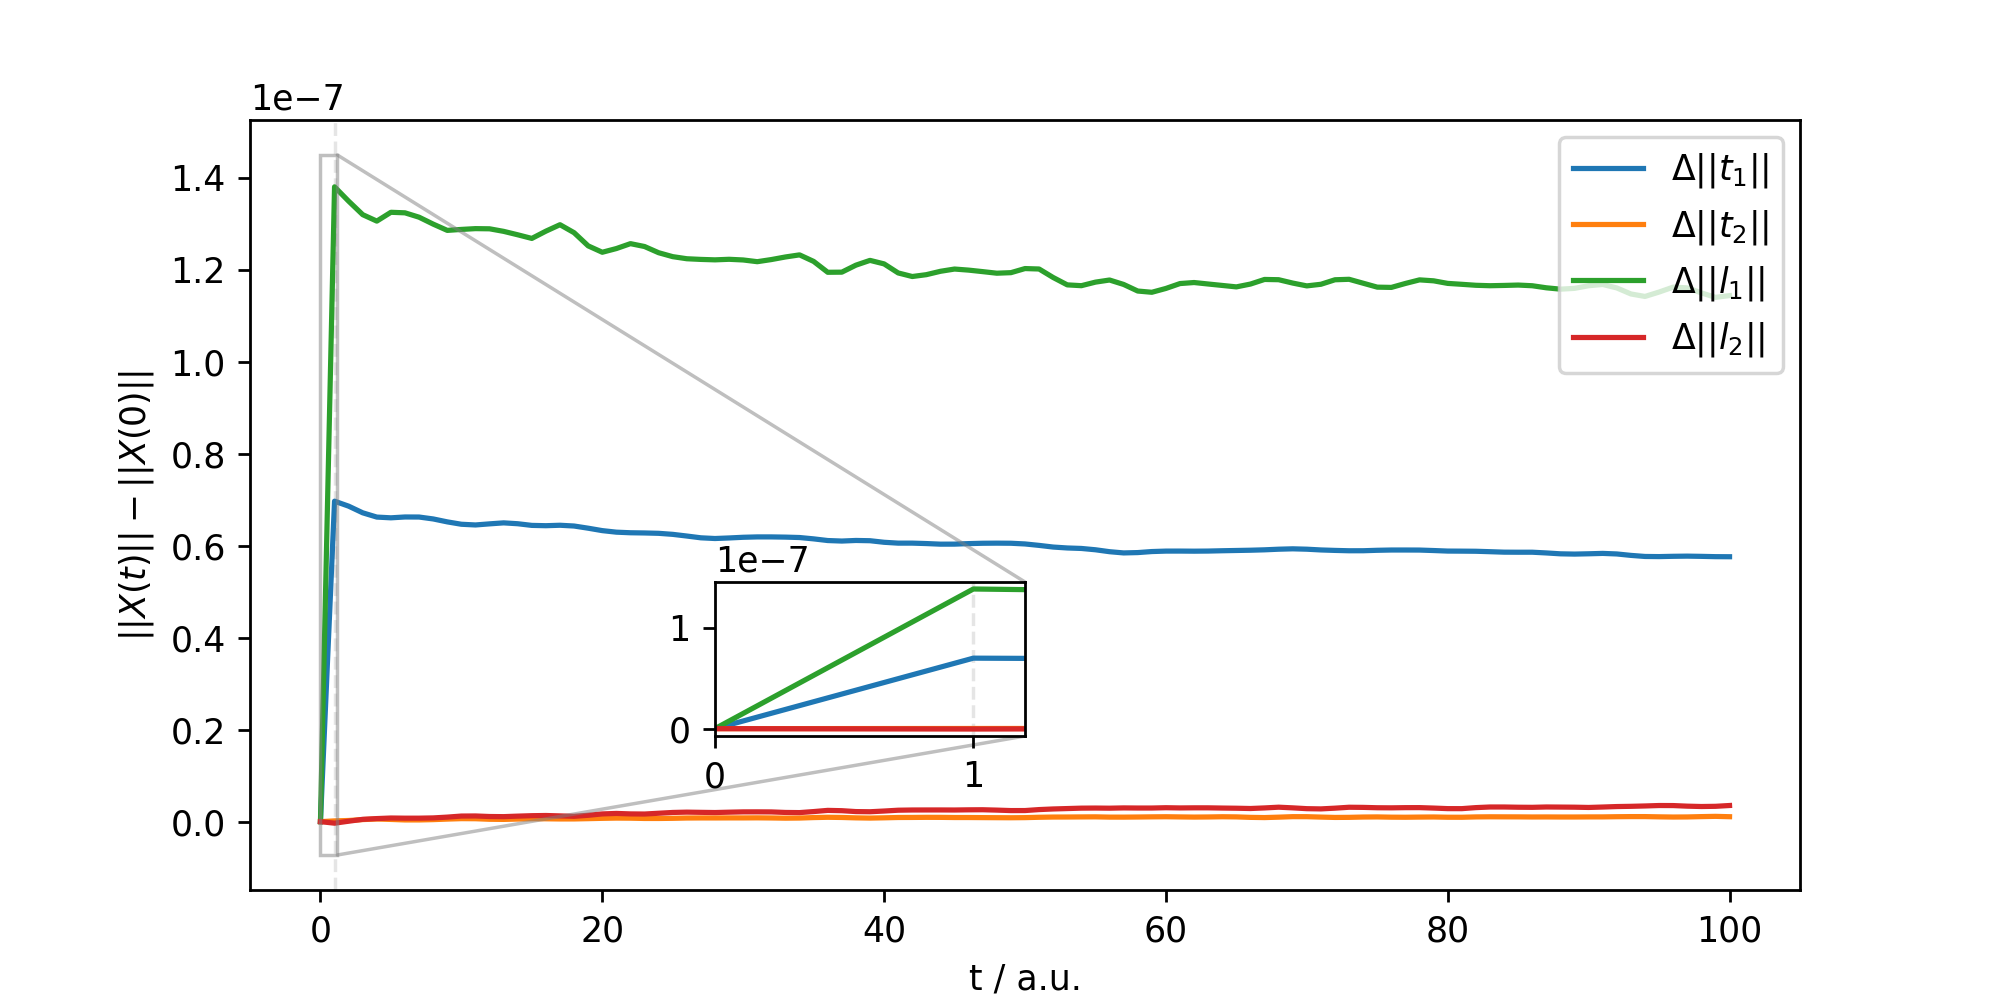
\includegraphics[scale=0.6]{p3/figures/si/pno_norm.png}
    \caption{Time-dependent change in the norm of the amplitude
    tensors relative to the ground-state amplitudes, using a PNO
    cut-off of $1\times10^{-9}$. (Amplitudes have been 
    back-transformed to the MO space for comparison to MO-basis
    amplitude norms. Field and step parameters remain unchanged,
    and the amplitude norm is taken at every 1 a.u.)}
    \label{fig:si:pno_norm}
\end{figure}
\begin{figure}
\centering
    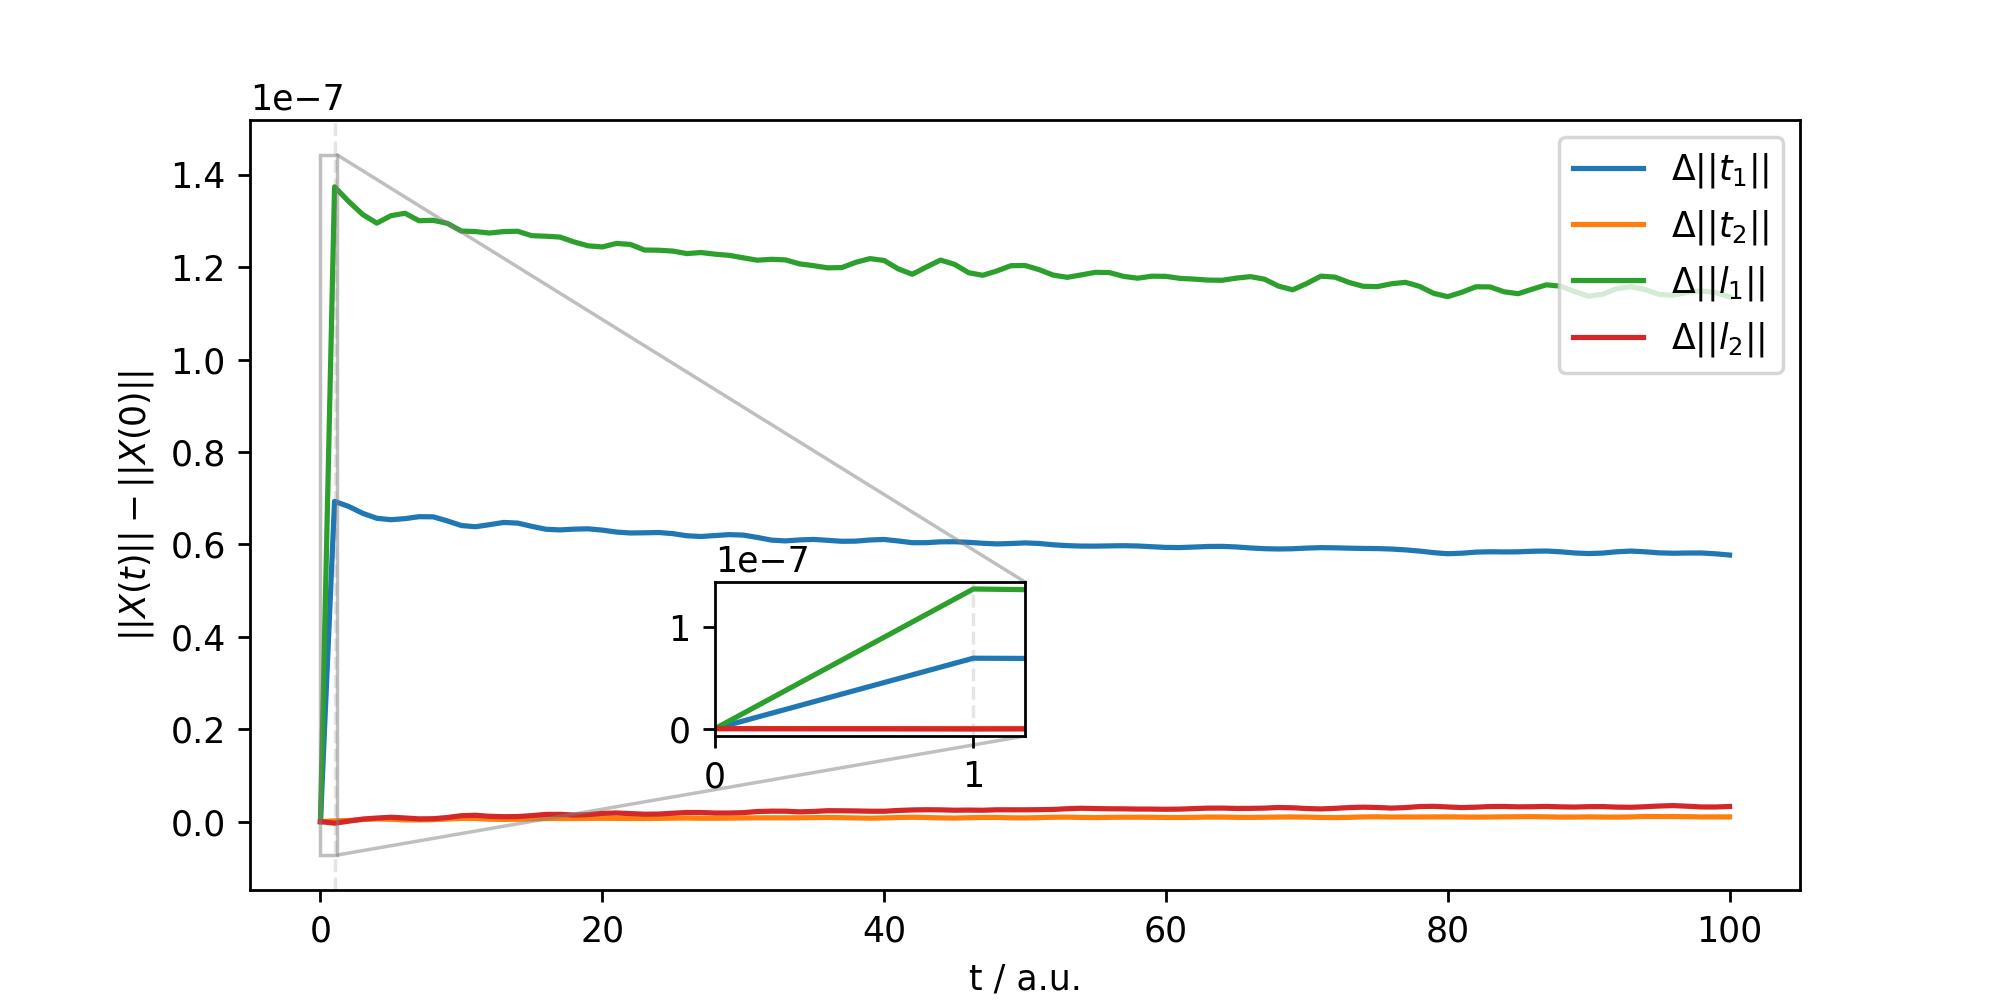
\includegraphics[scale=0.6]{p3/figures/si/pao_norm.png}
    \caption{Time-dependent change in the norm of the amplitude
    tensors relative to the ground-state amplitudes, using a PAO
    cut-off of $1\times10^{-3}$. (Amplitudes have been 
    back-transformed to the MO space for comparison to MO-basis
    amplitude norms. Field and step parameters remain unchanged,
    and the amplitude norm is taken at every 1 a.u.)}
    \label{fig:si:pao_norm}
\end{figure}
